\documentclass{standalone}
\usepackage{tikz}
\usetikzlibrary{decorations.pathmorphing}
\usetikzlibrary{decorations.markings}
\usetikzlibrary{calc}

%%%%%%%%%%%%%%%%%%%%%CODE FROM INTERNET FOR GRID WITH COORDIATES%%%%
\makeatletter
\def\grd@save@target#1{%
  \def\grd@target{#1}}
\def\grd@save@start#1{%
  \def\grd@start{#1}}
\tikzset{
  grid with coordinates/.style={
    to path={%
      \pgfextra{%
        \edef\grd@@target{(\tikztotarget)}%
        \tikz@scan@one@point\grd@save@target\grd@@target\relax
        \edef\grd@@start{(\tikztostart)}%
        \tikz@scan@one@point\grd@save@start\grd@@start\relax
        \draw[minor help lines] (\tikztostart) grid (\tikztotarget);
        \draw[major help lines] (\tikztostart) grid (\tikztotarget);
        \grd@start
        \pgfmathsetmacro{\grd@xa}{\the\pgf@x/1cm}
        \pgfmathsetmacro{\grd@ya}{\the\pgf@y/1cm}
        \grd@target
        \pgfmathsetmacro{\grd@xb}{\the\pgf@x/1cm}
        \pgfmathsetmacro{\grd@yb}{\the\pgf@y/1cm}
        \pgfmathsetmacro{\grd@xc}{\grd@xa + \pgfkeysvalueof{/tikz/grid with coordinates/major step}}
        \pgfmathsetmacro{\grd@yc}{\grd@ya + \pgfkeysvalueof{/tikz/grid with coordinates/major step}}
        \foreach \x in {\grd@xa,\grd@xc,...,\grd@xb}
        \node[anchor=north] at (\x,\grd@ya) {\pgfmathprintnumber{\x}};
        \foreach \y in {\grd@ya,\grd@yc,...,\grd@yb}
        \node[anchor=east] at (\grd@xa,\y) {\pgfmathprintnumber{\y}};
      }
    }
  },
  minor help lines/.style={
    help lines,
    step=\pgfkeysvalueof{/tikz/grid with coordinates/minor step}
  },
  major help lines/.style={
    help lines,
    line width=\pgfkeysvalueof{/tikz/grid with coordinates/major line width},
    step=\pgfkeysvalueof{/tikz/grid with coordinates/major step}
  },
  grid with coordinates/.cd,
  minor step/.initial=.2,
  major step/.initial=1,
  major line width/.initial=2pt,
}
\newcommand{\Ds}{\displaystyle}

\begin{document}
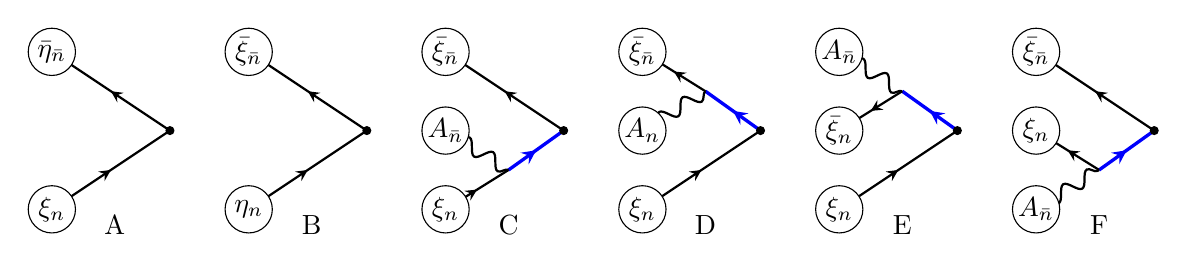
\begin{tikzpicture}
%\draw[step=.5cm] (0,0) to[grid with coordinates] (16,3);

%%%%%%%%%%%%%%%%%%%%%%%%%%%%%%%%%%%%%%%%%%%%%%%%%%%%%%%%%%%%%% diag-A
\coordinate (A) at (2, 1.5);

\draw[thick,postaction={decorate, decoration={
    markings,
    mark=at position 0.5 with {\arrow{stealth}}}}] ($(A)$)--($(A)+(-1.5,1.) $);
\draw[thick,postaction={decorate, decoration={
    markings,
    mark=at position 0.5 with {\arrow{stealth}}}}] ($(A)+(-1.5,-1.)$) -- ($(A)$);

\draw[fill=black] ($(A)$) circle (0.05cm);    
\draw[fill=white] ($(A)+(-1.5,-1.)$) circle (0.3cm);
\draw[fill=white] ($(A)+(-1.5,1.)$) circle (0.3cm);
\node[] at ($(A)+(-1.5,1.)$) {$\Ds\bar \eta_{\bar n}$};
\node[] at ($(A)+(-1.5,-1.)$) {$\Ds \xi_{n}$};
\node[] at ($(A)+(-0.7,-1.2)$) {A};

%%%%%%%%%%%%%%%%%%%%%%%%%%%%%%%%%%%%%%%%%%%%%%%%%%%%%%%%%%%%%% diag-B
\coordinate (A) at (4.5, 1.5);

\draw[thick,postaction={decorate, decoration={
    markings,
    mark=at position 0.5 with {\arrow{stealth}}}}] ($(A)$)--($(A)+(-1.5,1.) $);
\draw[thick,postaction={decorate, decoration={
    markings,
    mark=at position 0.5 with {\arrow{stealth}}}}] ($(A)+(-1.5,-1.)$) -- ($(A)$);

\draw[fill=black] ($(A)$) circle (0.05cm);    
\draw[fill=white] ($(A)+(-1.5,-1.)$) circle (0.3cm);
\draw[fill=white] ($(A)+(-1.5,1.)$) circle (0.3cm);
\node[] at ($(A)+(-1.5,1.)$) {$\Ds\bar \xi_{\bar n}$};
\node[] at ($(A)+(-1.5,-1.)$) {$\Ds \eta_{n}$};
\node[] at ($(A)+(-0.7,-1.2)$) {B};

%%%%%%%%%%%%%%%%%%%%%%%%%%%%%%%%%%%%%%%%%%%%%%%%%%%%%%%%%%%%%% diag-C
\coordinate (A) at (7, 1.5);

\draw[thick, postaction={decorate, decoration={
    markings,
    mark=at position 0.5 with {\arrow{stealth}}}}] ($(A)$)--($(A)+(-1.5,1.)$);
\draw[very thick, blue!99!black, postaction={decorate, decoration={
    markings,
    mark=at position 0.5 with {\arrow{stealth}}}}] ($(A)+(-0.7,-0.5)$)--($(A) $);
\draw[thick,postaction={decorate, decoration={
    markings,
    mark=at position 0.5 with {\arrow{stealth}}}}] ($(A)+(-1.5,-1.)$) -- ($(A)+(-0.7,-0.5)$);
\draw[thick,style={decorate, decoration=snake}] ($(A)+(-0.7,-0.5)$)--($(A)+(-1.5,0)$);

\draw[fill=black] ($(A)$) circle (0.05cm);    
\draw[fill=white] ($(A)+(-1.5,-1.)$) circle (0.3cm);
\draw[fill=white] ($(A)+(-1.5,+1)$) circle (0.3cm);
\draw[fill=white] ($(A)+(-1.5,0)$) circle (0.3cm);

\node[] at ($(A)+(-1.5,1.)$) {$\Ds\bar \xi_{\bar n}$};
\node[] at ($(A)+(-1.5,-1.)$) {$\Ds \xi_{n}$};
\node[] at ($(A)+(-1.5,0.)$) {$\Ds A_{\bar n}$};
\node[] at ($(A)+(-0.7,-1.2)$) {C};

%%%%%%%%%%%%%%%%%%%%%%%%%%%%%%%%%%%%%%%%%%%%%%%%%%%%%%%%%%%%%% diag-D
\coordinate (A) at (9.5, 1.5);


\draw[very thick, blue!99!black, postaction={decorate, decoration={
    markings,
    mark=at position 0.5 with {\arrow{stealth}}}}] ($(A)$)--($(A)+(-0.7,0.5)$);
\draw[thick,postaction={decorate, decoration={
    markings,
    mark=at position 0.5 with {\arrow{stealth}}}}] ($(A)+(-0.7,0.5)$)--($(A)+(-1.5,1.) $);
\draw[thick,postaction={decorate, decoration={
    markings,
    mark=at position 0.5 with {\arrow{stealth}}}}] ($(A)+(-1.5,-1.)$) -- ($(A)$);
\draw[thick,style={decorate, decoration=snake}] ($(A)+(-0.7,0.5)$)--($(A)+(-1.5,0)$);

\draw[fill=black] ($(A)$) circle (0.05cm);    
\draw[fill=white] ($(A)+(-1.5,-1.)$) circle (0.3cm);
\draw[fill=white] ($(A)+(-1.5,+1)$) circle (0.3cm);
\draw[fill=white] ($(A)+(-1.5,0)$) circle (0.3cm);

\node[] at ($(A)+(-1.5,1.)$) {$\Ds\bar \xi_{\bar n}$};
\node[] at ($(A)+(-1.5,-1.)$) {$\Ds \xi_{n}$};
\node[] at ($(A)+(-1.5,0.)$) {$\Ds A_{n}$};
\node[] at ($(A)+(-0.7,-1.2)$) {D};

%%%%%%%%%%%%%%%%%%%%%%%%%%%%%%%%%%%%%%%%%%%%%%%%%%%%%%%%%%%%%% diag-E
\coordinate (A) at (12, 1.5);

\draw[very thick, blue!99!black, postaction={decorate, decoration={
    markings,
    mark=at position 0.5 with {\arrow{stealth}}}}] ($(A)$)--($(A)+(-0.7,0.5)$);
\draw[thick,style={decorate, decoration=snake}] ($(A)+(-0.7,0.5)$)--($(A)+(-1.5,1.) $);
\draw[thick,postaction={decorate, decoration={
    markings,
    mark=at position 0.5 with {\arrow{stealth}}}}] ($(A)+(-1.5,-1.)$) -- ($(A)$);
\draw[thick,postaction={decorate, decoration={
    markings,
    mark=at position 0.5 with {\arrow{stealth}}}}] ($(A)+(-0.7,0.5)$)--($(A)+(-1.5,0)$);

\draw[fill=black] ($(A)$) circle (0.05cm);    
\draw[fill=white] ($(A)+(-1.5,-1.)$) circle (0.3cm);
\draw[fill=white] ($(A)+(-1.5,+1)$) circle (0.3cm);
\draw[fill=white] ($(A)+(-1.5,0)$) circle (0.3cm);

\node[] at ($(A)+(-1.5,1.)$) {$\Ds A_{\bar n}$};
\node[] at ($(A)+(-1.5,-1.)$) {$\Ds \xi_{n}$};
\node[] at ($(A)+(-1.5,0.)$) {$\Ds\bar \xi_{n}$};
\node[] at ($(A)+(-0.7,-1.2)$) {E};

%%%%%%%%%%%%%%%%%%%%%%%%%%%%%%%%%%%%%%%%%%%%%%%%%%%%%%%%%%%%%% diag-F
\coordinate (A) at (14.5, 1.5);

\draw[thick, postaction={decorate, decoration={
    markings,
    mark=at position 0.5 with {\arrow{stealth}}}}] ($(A)$)--($(A)+(-1.5,1.)$);
\draw[very thick, blue!99!black, postaction={decorate, decoration={
    markings,
    mark=at position 0.5 with {\arrow{stealth}}}}] ($(A)+(-0.7,-0.5)$)--($(A) $);
\draw[thick,style={decorate, decoration=snake}] ($(A)+(-1.5,-1.)$) -- ($(A)+(-0.7,-0.5)$);
\draw[thick,postaction={decorate, decoration={
    markings,
    mark=at position 0.5 with {\arrow{stealth}}}}] ($(A)+(-0.7,-0.5)$)--($(A)+(-1.5,0)$);

\draw[fill=black] ($(A)$) circle (0.05cm);    
\draw[fill=white] ($(A)+(-1.5,-1.)$) circle (0.3cm);
\draw[fill=white] ($(A)+(-1.5,+1)$) circle (0.3cm);
\draw[fill=white] ($(A)+(-1.5,0)$) circle (0.3cm);

\node[] at ($(A)+(-1.5,1.)$) {$\Ds\bar \xi_{\bar n}$};
\node[] at ($(A)+(-1.5,-1.)$) {$\Ds A_{\bar n}$};
\node[] at ($(A)+(-1.5,0.)$) {$\Ds \xi_{n}$};
\node[] at ($(A)+(-0.7,-1.2)$) {F};

\end{tikzpicture}
\end{document}